\documentclass[a4paper,12pt]{report}
% % % % % % % % % % % % % % % % % % % % % % % % % % % % % % % % %
% PACKAGES
% % % % % % % % % % % % % % % % % % % % % % % % % % % % % % % % %
\linespread{1.5}
\usepackage{amssymb}
\usepackage{amsmath}
\usepackage{verbatim}
\usepackage{graphicx}
\usepackage{color}
\usepackage{makeidx}
\usepackage{url}
\usepackage{enumitem}
\usepackage{sectsty}
\usepackage[T1]{fontenc}
\usepackage{lmodern}
\usepackage{booktabs}
\usepackage{tabularx}
\usepackage{hyperref}
\usepackage{parskip}
\usepackage{mathrsfs}
\usepackage{float}
\usepackage{placeins}
\usepackage{caption}
\usepackage{subcaption}
\chapterfont{\centering}
% % % % % % % % % % % % % % % % % % % % % % %
% ADJUSTMENT OF PAGES
% % % % % % % % % % % % % % % % % % % % % % %
\usepackage[top=2cm, bottom=2cm, left=3cm, right=2cm]{geometry}

% % % % % % % % % % % % % % % % % % % % % % % %
% SHORTCUTS
% % % % % % % % % % % % % % % % % % % % % % % %
\newtheorem{definition}{Definition}
\newtheorem{exm}{Example}
\newtheorem{exe}{Exercise}
\newtheorem{prob}{Problem}
\newtheorem{task}{TASK}
\newtheorem{theorem}{Theorem}
\newtheorem{proposition}{Proposition}
\newtheorem{proof}{Proof}
% % % % % % % % % % % % % % % % % % % % % % % % %
\renewcommand{\chaptername}{CHAPTER}
\renewcommand{\contentsname}{\centering CONTENTS}
\renewcommand{\listfigurename}{\centering LIST OF FIGURES}
\renewcommand{\listtablename}{\centering LIST OF TABLES}

\pagestyle{plain}
%==================================================================
\begin{document}
% % % % % % % % % % % % %
\pagenumbering{roman}
%===================================================================
%   Title page
%=====================================================================
{\large
\begin{center}
{\bf{Nonlinear Dynamics and Risk Quantification in Nepal Stock Exchange: A Jump-Diffusion COGARCH Approach}}\\
\end{center}

\vspace{0.8cm}

{\normalsize
\begin{center}
A FIRST YEAR PROJECT REPORT - MATH 562 II\\

\vspace{0.5cm}
SUBMITTED IN PARTIAL FULFILLMENT OF THE REQUIREMENTS FOR\\
THE DEGREE OF M.Sc. IN COMPUTATIONAL MATHEMATICS\\

\vspace{1.0cm}

BY
\end{center}
\begin{center}
\begin{itemize}
\begin{center}
Tek Raj Pant
\end{center}
\end{itemize}
\end{center}

\vspace{1.0cm}

\begin{figure}[htpb]
\centering

\includegraphics[height=4.5cm,width=4.5cm]{photos/kulogo.jpg}
\end{figure}

\vspace{2cm}
{\normalsize
\begin{center}
DEPARTMENT OF MATHEMATICS\\
SCHOOL OF SCIENCE\\
KATHMANDU UNIVERSITY\\
DHULIKHEL, NEPAL\\
\end{center}
}

\begin{center}
June 2026
\end{center}
}
}
\thispagestyle{empty}

%===================================================================
% Certificate and acknowledgement (placeholders)
\newpage



%\addcontentsline{toc}{chapter}{\bf Certification}
\addcontentsline{toc}{chapter}{\bf CERTIFICATION}

\begin{center}
	{\Large{\bf{ CERTIFICATION}}}
\end{center}


\noindent
This project entitled "Nonlinear Dynamics and Risk Quantification in Nepal Stock Exchange: A Jump-Diffusion COGARCH Approach" is carried out  under my supervision for the specified entire period satisfactorily, and is hereby certified as a work done by  \textbf{Tek Raj Pant} in partial fulfillment of the requirements for the degree of M.Sc. in Computational Mathematics, Department of Mathematics, Kathmandu University,  Dhulikhel, Nepal.

\vspace{2.0cm}


\noindent
-----------------------------\\
{\bf Dr. Samir Shrestha}\\
Associate Professor \\
Department of Mathematics,\\
School of Science, Kathmandu University,\\
Dhulikhel, Kavre, Nepal\\
Date:

\vspace{2cm}

\noindent
{\bf APPROVED BY:}\\
I hereby declare that the candidate qualifies to submit this  report of ------ 
to the Department of Mathematics. 


\noindent
-----------------------------\\
Prof. Dr. Rabindra Kayastha\\
Head of the Department\\
Department of Mathematics\\
School of Science\\
Kathmandu University\\
Date:
  

\newpage



%\addcontentsline{toc}{chapter}{\bf Acknowledgements}
\addcontentsline{toc}{chapter}{\bf ACKNOWLEDGEMENTS}
%{\Large{\bf{ACKNOWLEDGMENTS}}}\\

\begin{center}
	{\Large{\bf{ACKNOWLEDGMENTS}}}\\
\end{center}
\noindent
This research was carried out under the supervision of Dr. Samir Shrestha. I would like to express my sincere gratitude towards my supervisor for his excellent supervision, guidance and suggestion for accomplishing this work. And to the entire faculty of Department of Mathematics for encouraging, supporting and providing this opportunity.\\
\noindent
I am also thankful to my colleagues and the academic community at Kathmandu University for their constructive discussions and support during various stages of this research.
\noindent
I acknowledge the pioneering researchers in financial mathematics, stochastic calculus, and chaos theory whose foundational work made this research possible. Their contributions to understanding complex market dynamics provided the essential building blocks for this multi-model framework.
This research was conducted as part of the M.Sc. Computational Mathematics program at Kathmandu University.




%===================================================================
% Table of contents and lists
\tableofcontents

\listoftables
\addcontentsline{toc}{chapter}{LIST OF TABLES}

\newpage
\listoffigures
\addcontentsline{toc}{chapter}{LIST OF FIGURES}

%===================================================================
% LIST OF SYMBOLS
\newpage
\newpage
\addcontentsline{toc}{chapter}{\bf LIST OF SYMBOLS}

\begin{center}
{\LARGE{\bf{LIST OF SYMBOLS}}}
\end{center}

\begin{table}[H]
\centering
\begin{tabular}{p{2.5cm} p{8cm} p{4cm}}
\hline
\textbf{Symbol} & \textbf{Description} & \textbf{Context/Equation} \\
\hline
$S_t$ & Stock price at time $t$ & Main state variable \\
$V_t$ & Instantaneous variance (volatility) process & COGARCH process \\
$r_t$ & Daily log‑return & $r_t = \ln(S_t/S_{t-1})$ \\
$\alpha$ & Drift coefficient of the price process & Equation (1) \\
$W_t$ & Standard Brownian motion (continuous noise) & Equation (1) \\
$N_t$ & Poisson process with intensity $\lambda$ & Jump counting process \\
$Z$ & Jump size, $Z \sim \mathcal{N}(0,1)$ & Jump component \\
$\lambda$ & Daily jump probability (intensity parameter) & COGARCH, Table 3.1 \\
$\phi$ & Volatility feedback (jump sensitivity) parameter & Equation (2) \\
$\kappa$ & Mean reversion speed of volatility & Equation (2) \\
$\theta$ & Long‑run mean of the variance process & Equation (2) \\
$B$ & Branching ratio & $B = \frac{\lambda\phi\,\mathbb{E}[Z^2]}{\kappa}$ \\
$\gamma$ & Tail index (Hill estimator) & Measures tail heaviness of $|r_t|$ \\
$H$ & Hurst exponent (long‑memory indicator) & DFA on $|r_t|$ \\
$\Delta\alpha$ & Width of the multifractal spectrum & MF‑DFA, indicates multifractality \\
$\zeta(q)$ & Scaling function & $\zeta(q) = qH(q) - 1$ \\
$H(q)$ & Generalised Hurst exponent & MF‑DFA, varies with moment order $q$ \\
$f(\alpha)$ & Multifractal spectrum & Hölder exponent $\alpha$ vs. dimension $f(\alpha)$ \\
\hline
\end{tabular}
\caption{Core symbols used in the jump‑diffusion COGARCH framework and chaos diagnostics}
\label{tab:symbols1}
\end{table}

\begin{table}[H]
\centering
\begin{tabular}{p{2.5cm} p{8cm} p{4cm}}
\hline
\textbf{Symbol} & \textbf{Description} & \textbf{Context/Equation} \\
\hline
$\mathbb{E}[Z^2]$ & Second moment of jump size & For $Z\sim\mathcal{N}(0,1)$, $\mathbb{E}[Z^2]=1$ \\
$\omega$ & Base variance injection rate & $\omega = \kappa\theta$, GARCH(1,1) approximation \\
$\alpha_1$ & ARCH (shock sensitivity) coefficient & $\alpha_1 = \phi\lambda$ \\
$\beta_1$ & GARCH (persistence) coefficient & $\beta_1 = 1 - \kappa$ \\
$\hat{\gamma}$ & Estimated tail index & Hill estimator: $\hat{\gamma} = \frac{1}{k}\sum_{i=1}^{k}\ln\frac{X_{(i)}}{X_{(k+1)}}$ \\
$X_{(i)}$ & $i$-th order statistic of $|r_t|$ & Used in Hill estimator \\
$k$ & Number of upper order statistics & Typically $5\%$ of sample \\
$F_q(n)$ & $q$-th order fluctuation function & MF‑DFA \\
$q$ & Moment order in multifractal analysis & MF‑DFA, $q\in[-5,5]\setminus\{0\}$ \\
$T$ & Total number of observations & Post‑break sample: $T=2886$ \\
$\lambda_{\text{annual}}$ & Annualised jump intensity & $\lambda_{\text{annual}} = \lambda \times 252$ \\
\hline
\end{tabular}
\caption{Secondary symbols and estimation quantities}
\label{tab:symbols2}
\end{table}

\begin{table}[H]
\centering
\begin{tabular}{p{2.5cm} p{8cm} p{4cm}}
\hline
\textbf{Symbol} & \textbf{Description} & \textbf{Context/Equation} \\
\hline
$\text{VaR}_p$ & Value‑at‑Risk at confidence level $p$ & Risk measure: $p=0.95,0.99$ \\
$\text{CVaR}_p$ & Conditional VaR (Expected Shortfall) & Average loss beyond VaR$_p$ \\
$\text{ACF}$ & Autocorrelation function & Used on $r_t$ and $|r_t|$ \\
$\text{PACF}$ & Partial autocorrelation function & Used for mean equation specification \\
$\text{DFA}$ & Detrended fluctuation analysis & Estimates Hurst exponent $H$ \\
$\text{MF‑DFA}$ & Multifractal DFA & Estimates $H(q)$ and $\Delta\alpha$ \\
$\text{MSM}$ & Method of Simulated Moments & Estimation procedure for COGARCH \\
$\text{ADF}$ & Augmented Dickey–Fuller test & Stationarity test (unit root null) \\
$\text{KPSS}$ & Kwiatkowski–Phillips–Schmidt–Shin test & Stationarity test (stationary null) \\
$\text{LB}$ & Ljung–Box $Q$‑test & Test for serial correlation \\
$\text{ARCH LM}$ & Engle’s ARCH Lagrange multiplier test & Test for conditional heteroskedasticity \\
\hline
\end{tabular}
\caption{Acronyms and risk measures}
\label{tab:symbols3}
\end{table}

%===================================================================
\newpage
\pagenumbering{arabic}

% ===============================
% CHAPTER 1: INTRODUCTION
% ===============================
\chapter{INTRODUCTION}

\section{Background}
Empirical studies show that stock markets exhibit sudden shocks and persistent volatility \cite{duong2010empirical}. For emerging markets like the Nepal Stock Exchange (NEPSE), these features are amplified by thin liquidity, political uncertainty, and external shocks \cite{worldbank2020nepal}. Traditional models based on constant volatility and continuous paths fail to capture the observed leptokurtic returns and volatility clustering.

Theoretical framework \cite{kluppelberg2004continuous} couples a jump‑diffusion price process with a continuous‑time GARCH (COGARCH) volatility feedback. This model possesses an internal self‑exciting mechanism that, in a near‑critical branching regime, produces patterns indistinguishable from deterministic chaos with heavy‑tailed volatility, long memory, and multifractal scaling. The model provides us with falsifiable conditions linking these “chaotic” signatures to a branching ratio $B$, a tail index $\gamma$, and the Hurst exponent $H$. This paper attempts to find out those theoretical predictions to empirical scrutiny using real data from the NEPSE banking sector.

\section{Problem Statement}
The theoretical jump‑diffusion COGARCH model states that when the branching ratio $B$ approaches $1$ from below, the volatility process enters a near‑critical state characterised by:
\begin{enumerate}[label=(\roman*)]
    \item a tail index $\gamma \le 2$ (infinite variance of volatility),
    \item a Hurst exponent $H > 0.5$ for absolute returns (long memory),
    \item non‑linear scaling $\zeta(q)$ in the moment structure (multifractality).
\end{enumerate}
These conditions constitute a set of falsifiable hypotheses. The present study asks: \emph{Do daily returns from the NEPSE banking sector satisfy these conditions?} If so, the model is validated and can be used for risk quantification, if not, the critical branching hypothesis is rejected for NEPSE.

\section{Literature Review}
The literature on jump‑diffusion and stochastic volatility has been comprehensively reviewed in \cite{kluppelberg2004continuous}. Key developments include Merton’s jump‑diffusion \cite{merton1976option}, the GARCH family \cite{engle1982autoregressive, bollerslev1986generalized}, and the continuous‑time COGARCH \cite{kluppelberg2004continuous}. The application of chaos theory to financial markets gained traction after Peters \cite{peters1994fractal}, while Mandelbrot’s fractal geometry \cite{mandelbrot2013fractals} and the multifractal model of asset returns \cite{calvet2002multifractality} provided tools to detect scaling behaviour. Hardiman et al.\ \cite{hardiman2013critical} demonstrated that developed markets operate near a critical branching ratio $B \approx 1$, but similar tests in emerging markets remain scarce. Studies on NEPSE have largely focused on simple GARCH models \cite{gajurel2021volatility} without exploring jump‑driven feedback or chaotic diagnostics. This study bridges that gap by conducting a full empirical validation of the jump‑diffusion COGARCH framework in NEPSE.

\section{Objectives}
The study is organised around the following objectives:
\begin{enumerate}[label=(\roman*)]
    \item Conduct exploratory data analysis (EDA) of NEPSE banking sector returns.
    \item Estimate the continuous‑time COGARCH parameters using the Method of Simulated Moments (MSM) with a discrete GARCH‑jump approximation.
    \item Compute chaos diagnostics (branching ratio $B$, tail index $\gamma$, Hurst exponent $H$, multifractal width $\Delta\alpha$) and compare them with theoretical thresholds.
    \item Quantify one‑year ahead risk measures (VaR, CVaR, drawdown probabilities) via Monte Carlo simulation of the fitted model.
\end{enumerate}

\section{Scope and Limitations}
This study is confined to the \textbf{Commercial Banks} sector index of NEPSE, using daily closing prices(index) from 1 October 2013 to 3 June 2026 ($T=2886$ observations). The start date is chosen as the endogenous break point identified using Zivot–Andrews test. The study focuses on model validation and risk simulation. It does not extend to high‑frequency data and multivariate settings.

Limitations include:
\begin{enumerate}[label=(\roman*)]
    \item Daily data may miss intraday jumps, potentially and can have bias for jump intensity estimates.
    \item The Poisson assumption with constant intensity $\lambda$ may be restrictive, more robust Hawkes process could better capture clustering.
    \item The discrete‑time approximation used in MSM introduces a mapping error from the continuous COGARCH.
    \item Results from the banking sector may not generalize to other sectors or the overall market, but we can use this framework for other sectors as well.
\end{enumerate}

% ===============================
% SECTION: MATHEMATICAL PRELIMINARIES (within a chapter, e.g., after INTRODUCTION)
% ===============================
\section{MATHEMATICAL PRELIMINARIES}

This section provides an overview of the statistical, econometric, and chaos‑theoretic concepts used throughout the study. Each method is briefly described, and the relevant test statistics or estimators are defined.

\subsection{Distributional Diagnostics}

\subsubsection{Skewness and Excess Kurtosis}
Skewness measures the asymmetry of a distribution:
\[
\text{Skewness} = \frac{\mathbb{E}[(X-\mu)^3]}{\sigma^3}.
\]
Positive skewness indicates a longer right tail. Excess kurtosis measures tail heaviness:
\[
\text{Excess Kurtosis} = \frac{\mathbb{E}[(X-\mu)^4]}{\sigma^4} - 3.
\]
A normal distribution has excess kurtosis zero; positive values indicate heavy tails (leptokurtosis).

\subsubsection{Jarque–Bera Test}
The Jarque–Bera (JB) test assesses whether a sample comes from a normal distribution. It uses sample skewness \(S\) and excess kurtosis \(K\):
\[
\text{JB} = \frac{n}{6}\left(S^2 + \frac{K^2}{4}\right),
\]
where \(n\) is the sample size. Under the null hypothesis of normality, JB follows a \(\chi^2\) distribution with 2 degrees of freedom.

\subsubsection{Shapiro–Wilk Test}
The Shapiro–Wilk test is a powerful omnibus test for normality. The statistic is
\[
W = \frac{\left(\sum_{i=1}^{n} a_i x_{(i)}\right)^2}{\sum_{i=1}^{n} (x_i - \bar{x})^2},
\]
where \(x_{(i)}\) are the ordered sample values and \(a_i\) are coefficients generated from the order statistics of a standard normal. Small values of \(W\) indicate non‑normality.

\subsubsection{Quantile-Quantile (Q-Q) Plot}
A Q-Q plot compares the empirical quantiles of a sample against the theoretical quantiles of a specified distribution (e.g., normal). If the points lie approximately on the 45° line, the sample is consistent with the theoretical distribution. Deviations in the tails indicate heavier or lighter tails than the normal.

\subsection{Time Series Dependence Tests}

\subsubsection{Ljung–Box Q-test}
The Ljung–Box test checks for autocorrelation in a time series up to a specified lag \(h\). The test statistic is
\[
Q_h = n(n+2) \sum_{k=1}^{h} \frac{\hat{\rho}_k^2}{n-k},
\]
where \(\hat{\rho}_k\) is the sample autocorrelation at lag \(k\). Under the null hypothesis of no serial correlation (white noise), \(Q_h \sim \chi^2_h\).

\subsubsection{Engle’s ARCH Lagrange Multiplier (LM) Test}
This test detects autoregressive conditional heteroskedasticity (ARCH). It regresses the squared residuals on their own lags:
\[
\hat{\varepsilon}_t^2 = \alpha_0 + \alpha_1 \hat{\varepsilon}_{t-1}^2 + \cdots + \alpha_p \hat{\varepsilon}_{t-p}^2 + u_t.
\]
The LM statistic is \(nR^2\) under the null of no ARCH (\(\alpha_1 = \cdots = \alpha_p = 0\)), asymptotically distributed as \(\chi^2_p\).

\subsection{Stationarity Tests}

\subsubsection{Augmented Dickey–Fuller (ADF) Test}
The ADF test examines for a unit root. The regression is
\[
\Delta y_t = \beta_0 + \beta_1 t + \gamma y_{t-1} + \sum_{i=1}^{p} \delta_i \Delta y_{t-i} + \varepsilon_t.
\]
The null hypothesis is \(\gamma = 0\) (unit root). Rejection indicates stationarity.

\subsubsection{KPSS Test}
The KPSS test has the null hypothesis that the series is stationary (trend‑stationary). The test statistic is based on the partial sum of residuals. A small p‑value (\(<0.05\)) rejects stationarity.

\subsection{Jump Detection and Structural Break}

\subsubsection{Dynamic \(3\sigma\) Filter}
A rolling window of length \(w\) (e.g., 21 days) is used to compute the local mean \(\mu_t\) and standard deviation \(\sigma_t\). An observation is flagged as a jump if
\[
|r_t - \mu_t| > 3\sigma_t.
\]

\subsubsection{Zivot–Andrews Test}
This test allows for one endogenous structural break in the level or trend of a time series under the unit‑root null. The test statistic is the minimum \(t\)-statistic over all possible break dates. A break date is chosen where the test statistic is most negative.

\subsection{Chaos Diagnostics}

\subsubsection{Hill Tail Index}
The Hill estimator estimates the tail index \(\gamma\) of a heavy‑tailed distribution. For the top \(k\) order statistics of absolute returns \(|r_t|\):
\[
\hat{\gamma} = \frac{1}{k} \sum_{i=1}^{k} \ln\left(\frac{X_{(i)}}{X_{(k+1)}}\right),
\]
where \(X_{(1)} \ge X_{(2)} \ge \cdots\) are the sorted absolute returns.

\subsubsection{Detrended Fluctuation Analysis (DFA)}
DFA quantifies long‑memory in non‑stationary time series. The integrated series is divided into boxes of length \(n\). A polynomial trend is removed, and the fluctuation function \(F(n)\) is computed. The Hurst exponent \(H\) is the slope of \(\log F(n)\) versus \(\log n\).  
\(H = 0.5\): uncorrelated (white noise); \(H > 0.5\): persistent (long memory); \(H < 0.5\): anti‑persistent.

\subsubsection{Multifractal Detrended Fluctuation Analysis (MF‑DFA)}
MF‑DFA generalises DFA by considering different moment orders \(q\). The \(q\)-th order fluctuation function is
\[
F_q(n) = \left( \frac{1}{N_n} \sum_{\nu=1}^{N_n} \left[ F^2(\nu,n) \right]^{q/2} \right)^{1/q},
\]
where \(F^2(\nu,n)\) is the variance in box \(\nu\). The generalised Hurst exponent \(H(q)\) is obtained from \(F_q(n) \propto n^{H(q)}\). The scaling function is \(\zeta(q) = qH(q) - 1\). Non‑linear \(\zeta(q)\) indicates multifractality. The multifractal spectrum \(f(\alpha)\) is related to \(H(q)\) via a Legendre transform, and its width \(\Delta\alpha = \alpha_{\max} - \alpha_{\min}\) quantifies the degree of multifractality.

\subsection{COGARCH Model and Estimation}

\subsubsection{Jump‑Diffusion COGARCH Model}
The continuous‑time model is given by
\begin{align}
\frac{dS_t}{S_{t-}} &= \alpha\,dt + \sqrt{V_{t-}}\,dW_t + \bigl(e^{\sqrt{V_{t-}}Z} - 1\bigr)\,dN_t, \\
dV_t &= \kappa(\theta - V_{t-})\,dt + \phi\, V_{t-}\,Z^2\,dN_t,
\end{align}
with \(W_t\) Brownian motion, \(N_t\) Poisson process (intensity \(\lambda\)), and \(Z\sim\mathcal{N}(0,1)\).

\subsubsection{Branching Ratio}
\[
B = \frac{\lambda\,\phi\,\mathbb{E}[Z^2]}{\kappa}.
\]
When \(B \lesssim 1\), the volatility process is near‑critical, exhibiting long memory and multifractality.

\subsubsection{Method of Simulated Moments (MSM)}
MSM estimates parameters by minimising the weighted distance between empirical moments and moments computed from simulated data:
\[
\hat{\theta} = \arg\min_{\theta} \left( m_{\text{emp}} - m_{\text{sim}}(\theta) \right)' W \left( m_{\text{emp}} - m_{\text{sim}}(\theta) \right).
\]
Moments include mean, variance, skewness, kurtosis, autocorrelations of \(|r_t|\), and the Hill tail index.

\subsection{Risk Measures}

\subsubsection{Value‑at‑Risk (VaR)}
VaR at confidence level \(p\) (e.g., 95\%) is the \(p\)-th percentile of the return distribution:
\[
\text{VaR}_p = \inf\{ x \mid F(x) \ge p \}.
\]

\subsubsection{Conditional VaR (CVaR)}
CVaR, also called Expected Shortfall, is the expected loss given that the loss exceeds VaR:
\[
\text{CVaR}_p = \mathbb{E}[\,X \mid X \le \text{VaR}_p\,].
\]

\subsubsection{Maximum Drawdown}
For a price path \(P_t\), the maximum drawdown is the largest peak‑to‑trough decline:
\[
\text{MDD} = \max_{0 \le s \le t \le T} \left( \frac{P_s - P_t}{P_s} \right).
\]
% ===============================
% CHAPTER 2: DATA AND EXPLORATORY ANALYSIS
% ===============================
\chapter{Data and Exploratory Analysis}

\section{Data Description}
We use daily closing prices of the \textbf{Commercial Banks} sector index of the NEPSE. The raw data is from 1 January 2012 to 3 June 2026, but using the Zivot–Andrews test, an endogenous structural break was detected on 30 September 2013 (see Section \ref{sec:break}), so we restrict the analysis to the period from 1 October 2013 to 3 June 2026, yielding $T = 2886$ daily observations. Log‑returns are computed as $r_t = \ln(P_t / P_{t-1})$.

\section{Distributional Diagnostics}
Table \ref{tab:desc} has the descriptive statistics of the daily log‑returns. The mean is close to zero, but positive ($0.0424\%$), and the standard deviation is $1.53\%$. The skewness of $0.9029$ indicates a right‑tailed distribution, and the excess kurtosis of $7.2073$ is confirmation of heavy tails. Formal normality tests (Jarque–Bera and Shapiro–Wilk) decisively reject the null of normality ($p<0.0001$).

Figure \ref{fig:density} overlays the empirical return density with a theoretical Gaussian distribution. The histogram shows a sharp central peak (leptokurtosis) and fatter tails than the normal curve, visually confirming the excess kurtosis reported in Table \ref{tab:desc}. 

\begin{figure}[H]
\centering
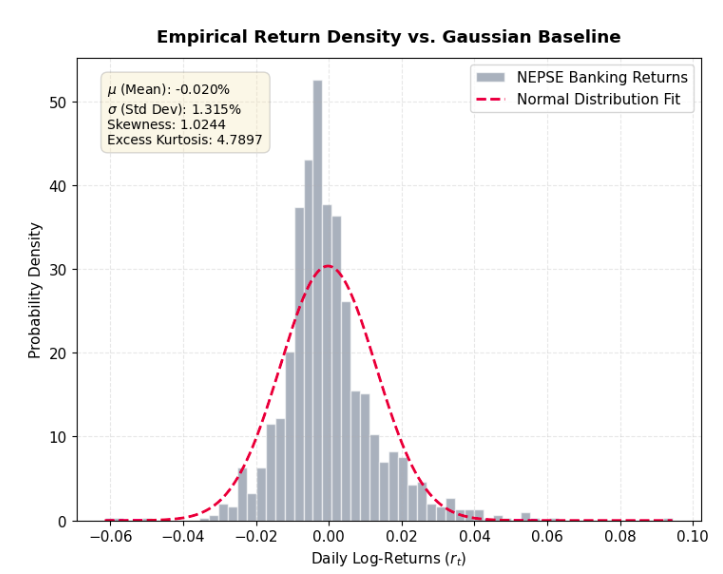
\includegraphics[width=0.8\textwidth]{figures/emperical-vs-gaussian.png}
\caption{Empirical return density vs. Gaussian baseline (leptokurtic peak).}
\label{fig:density}
\end{figure}

Figure \ref{fig:qq} (normal Q-Q plot) further highlights tail deviations: the sample quantiles depart from the 45° reference line, with extreme positive and negative returns lying far outside the Gaussian confidence bands. These empirical facts motivate the use of jump‑diffusion model.

\begin{figure}[H]
\centering
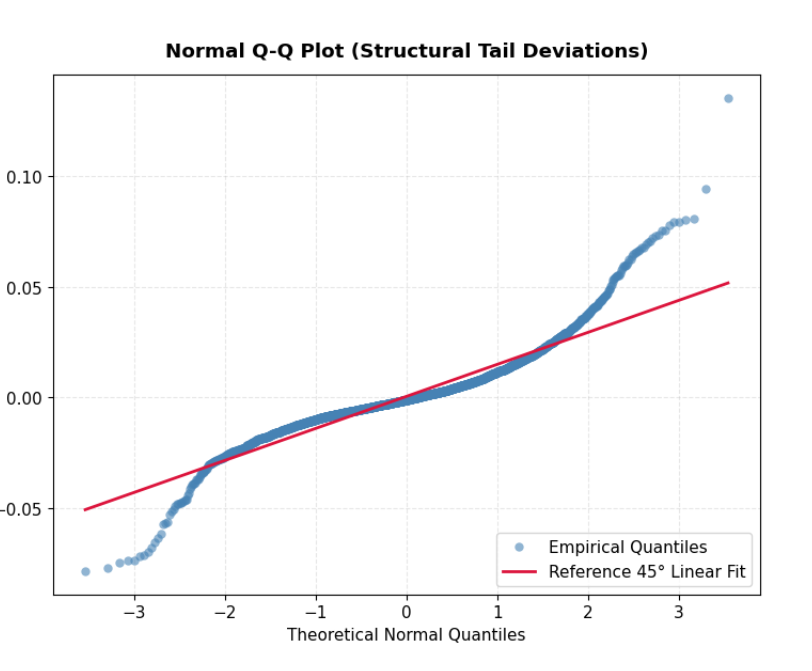
\includegraphics[width=0.8\textwidth]{figures/normal-q-q.png}
\caption{Normal Q-Q plot showing tail deviations.}
\label{fig:qq}
\end{figure}

\begin{table}[H]
\centering
\caption{Descriptive statistics and normality tests for NEPSE Commercial Banks daily log‑returns (October 2013 – June 2026).}
\label{tab:desc}
\begin{tabular}{l r}
\toprule
Statistic & Value \\
\midrule
Mean (daily) & $0.000424$ ($0.0424\%$) \\
Variance (daily) & $0.000235$ \\
Std. deviation (daily) & $0.015321$ ($1.5321\%$) \\
Skewness & $0.9029$ \\
Excess kurtosis & $7.2073$ \\
Jarque–Bera test & Stat $= 7981.75$, $p = 0.0000$ \\
Shapiro–Wilk test & Stat $= 0.8919$, $p = 0.0000$ \\
\bottomrule
\end{tabular}
\end{table}

\section{Time Series Dependence and ARCH Effects}
\paragraph{Serial correlation.}
The Ljung–Box test on raw returns (Table \ref{tab:serial}) shows significant autocorrelation at lags 10 and 20 ($p<0.001$), indicating that the mean equation requires an autoregressive structure. Squared returns exhibit even stronger dependence, with test statistics that are orders of magnitude larger and $p$-values virtually zero – clear evidence of volatility clustering.

\paragraph{ARCH effects.}
Engle’s ARCH Lagrange Multiplier test (lag 10) gives a statistic of $778.07$ ($p=1.07\times10^{-160}$), strongly rejecting the null of no conditional heteroskedasticity. This establishes a firm baseline for GARCH‑type variance dynamics.

Figure \ref{fig:acfpacf} displays the autocorrelation (ACF) and partial autocorrelation (PACF) of raw returns (top row) and squared returns (bottom row). For raw returns, only a few lags exceed the significance bands, suggesting weak but non‑negligible serial correlation. In contrast, the ACF of squared returns decays very slowly, remaining positive for more than 30 lags – a classic signature of long‑memory volatility clustering. The PACF of squared returns cuts off after a few lags, supporting an ARCH/GARCH specification.

\begin{figure}[H]
\centering
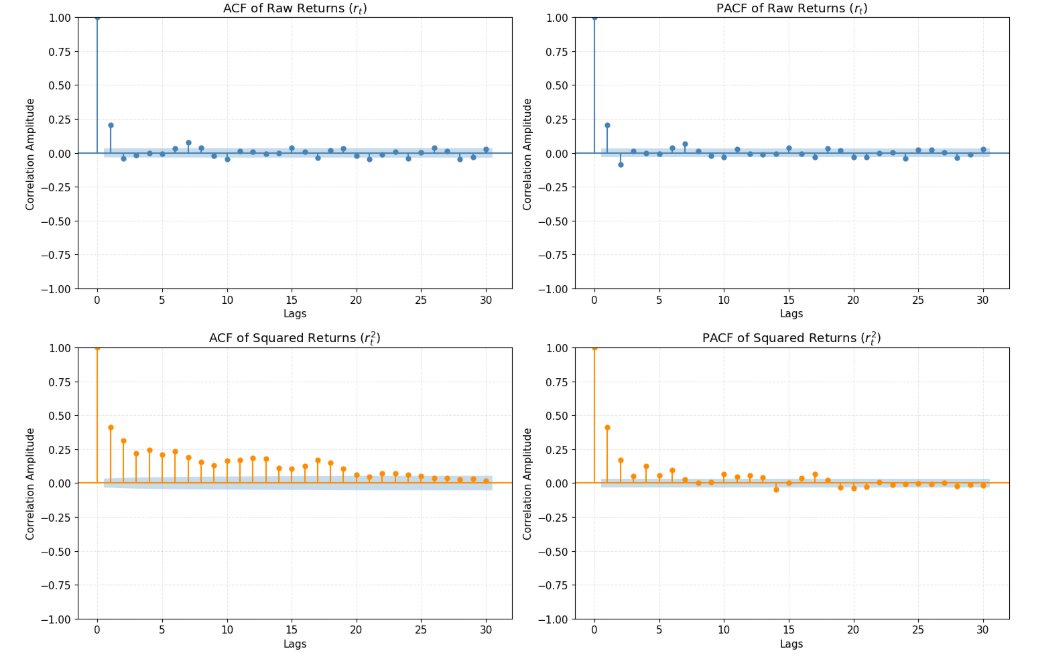
\includegraphics[width=0.8\textwidth]{figures/acf-pacf.png}
\caption{ACF and PACF of raw returns (mean equation) and squared returns (variance equation).}
\label{fig:acfpacf}
\end{figure}

Figure \ref{fig:volcluster} shows the raw log-returns with a rolling 21-day volatility corridor, visually confirming the alternating calm and turbulent periods characteristic of volatility clustering.

\begin{figure}[H]
\centering
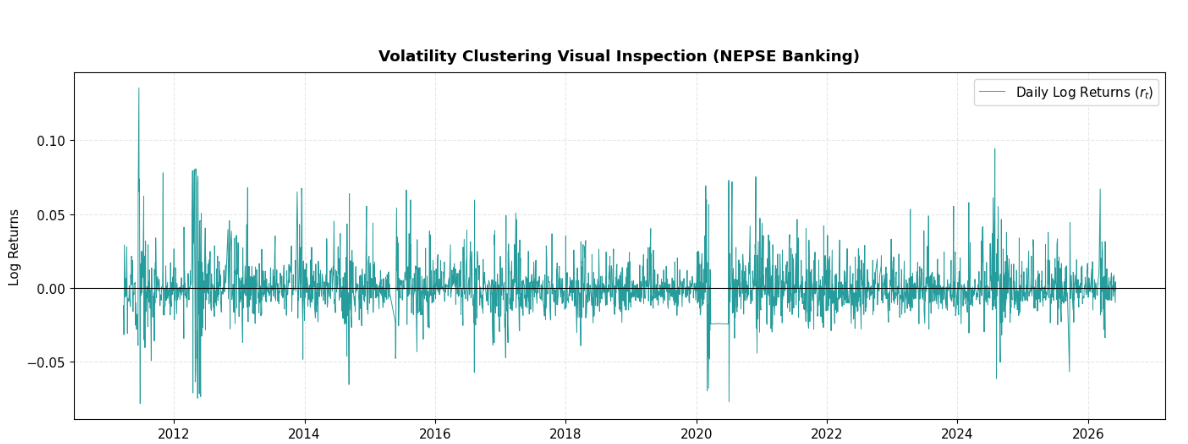
\includegraphics[width=0.8\textwidth]{figures/volatility-clustering-visual-inspection.png}
\caption{Volatility clustering visual inspection (log returns with 21‑day rolling volatility corridor).}
\label{fig:volcluster}
\end{figure}

\begin{table}[H]
\centering
\caption{Ljung–Box and ARCH tests for raw and squared returns (post‑break sample).}
\label{tab:serial}
\begin{tabular}{l c c}
\toprule
Test & Statistic & $p$-value \\
\midrule
LB (raw returns, lag 10) & $190.69$ & $0.0000$ \\
LB (raw returns, lag 20) & $208.99$ & $0.0000$ \\
LB (squared returns, lag 10) & $2015.56$ & $0.0000$ \\
LB (squared returns, lag 20) & $2720.19$ & $0.0000$ \\
Engle ARCH LM (lag 10) & $778.07$ & $0.0000$ \\
\bottomrule
\end{tabular}
\end{table}

\paragraph{Leverage effect.}
We examined the cross‑correlation between past returns $r_{t-k}$ and current absolute returns $|r_t|$ for $k=1,\dots,20$ days. The minimum correlation is $0.0088$ at lag 9, which lies inside the 95\% asymptotic confidence band $\pm 0.0333$. Hence no statistically significant leverage effect is present; negative and positive shocks have symmetric impacts on future volatility. A symmetric GARCH specification is therefore admissible.

\section{Stationarity and Ergodicity}
The Augmented Dickey–Fuller (ADF) test yields a statistic of $-11.4461$ ($p=6.01\times10^{-21}$), rejecting the unit‑root null. The KPSS test gives a statistic of $0.2225$ ($p>0.1$), failing to reject stationarity. Together, these results confirm that the log‑return series is strictly stationary and mean‑reverting, providing a solid foundation for time series modelling.

\section{Jump Detection and Structural Break}
\label{sec:break}
\paragraph{Jump identification.}
We apply a dynamic $3\sigma$ filter using a rolling 21‑day window to isolate outlier shocks. Figure \ref{fig:jumps} illustrates the detected jumps (red dots) against the daily log‑returns (grey line) and the rolling $3\sigma$ corridor (orange dashed). The plot shows that most large positive or negative returns are flagged as jumps, and these jumps are often followed by periods of elevated volatility. A total of $39$ jump events are detected, corresponding to $1.12\%$ of trading days. The annualised jump intensity (based on 252 trading days) is $\lambda_{\text{annual}} = 2.83$ jumps per year. The mean inter‑arrival time between jumps is $88.4$ trading days (median $75.5$ days), indicating that jumps occur roughly every four months.

\begin{figure}[H]
\centering
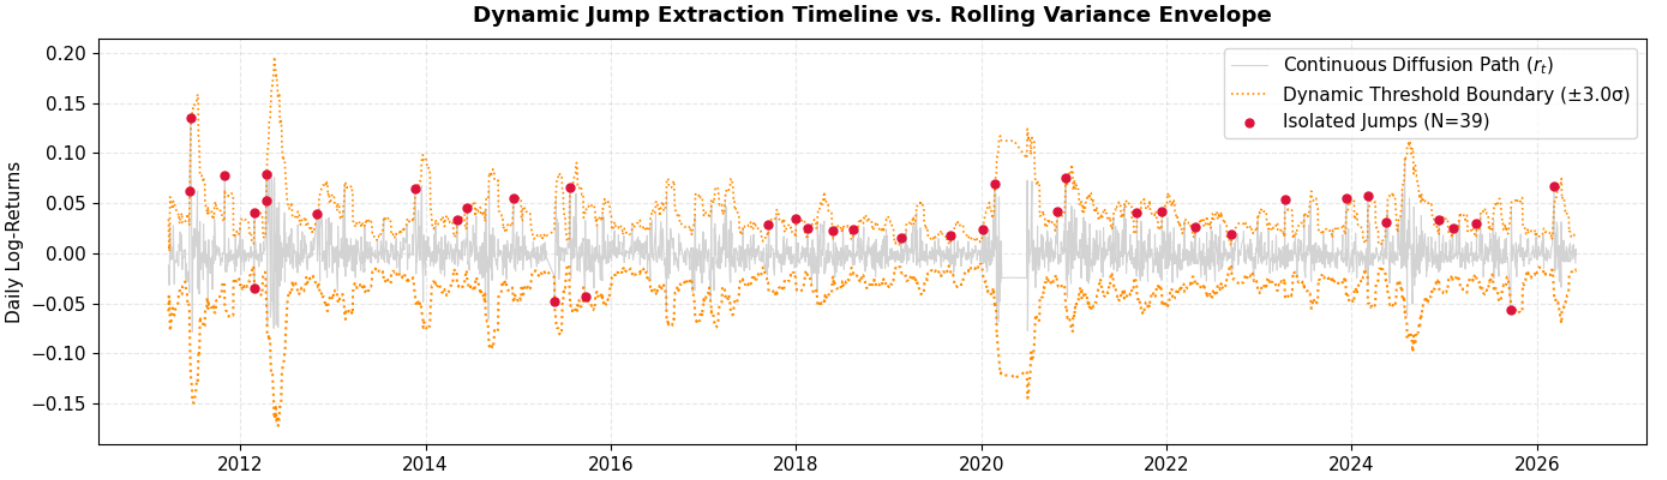
\includegraphics[width=0.8\textwidth]{figures/dynamic-jump.png}
\caption{Dynamic jump extraction timeline (rolling $3\sigma$ corridor and detected jumps).}
\label{fig:jumps}
\end{figure}

\paragraph{Structural break analysis.}
The Zivot–Andrews test on log prices (with one endogenous break) produces a test statistic of $-3.1718$ ($p=0.852$), failing to reject the unit‑root null. The estimated break date is \textbf{30 September 2013}. Figure \ref{fig:break} shows the log‑price series with a vertical line at the break point. While the test does not find a permanent regime shift, the break point is used to define a homogeneous sample for COGARCH estimation, as the pre‑break period (2012–2013) exhibits different dynamics. All subsequent analyses are therefore conducted on the post‑break sample (1 October 2013 – 3 June 2026).

\begin{figure}[H]
\centering
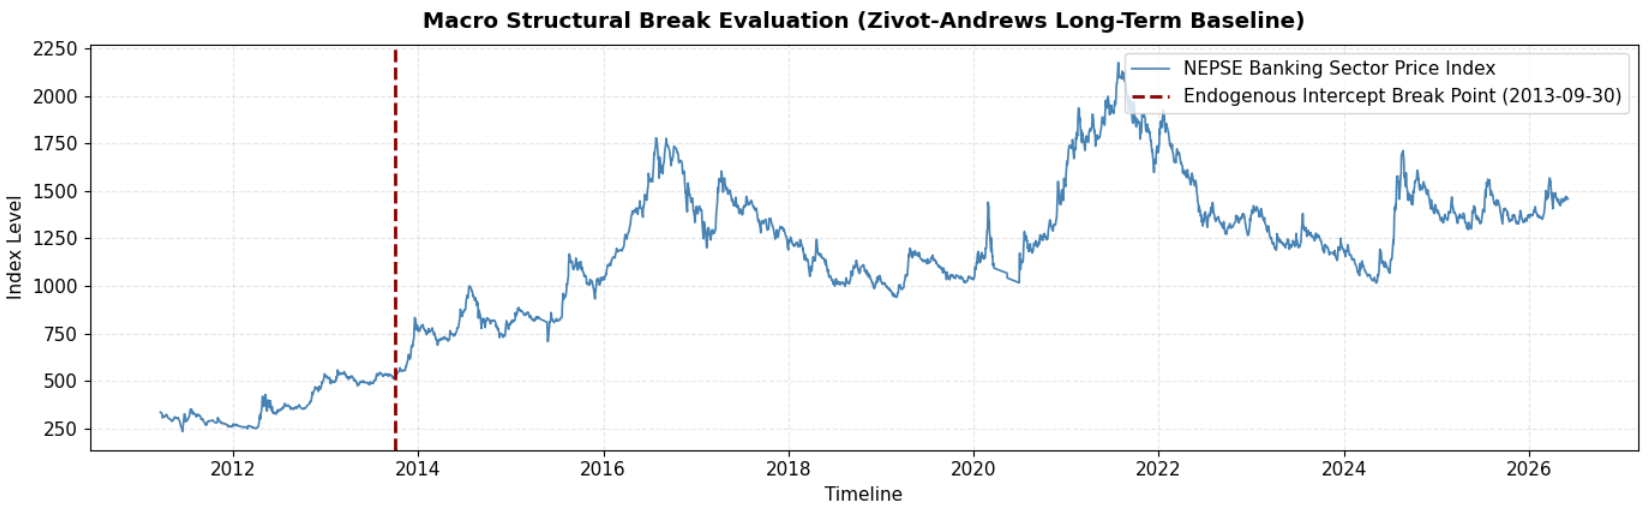
\includegraphics[width=0.8\textwidth]{figures/breakdown.png}
\caption{Macro Structural Break Evaluation (Zivot-Andrews Long-Term Baseline).}
\label{fig:break}
\end{figure}

\section{Empirical Chaos Diagnostics (Post‑Break Sample)}
\paragraph{Tail index.}
The Hill estimator applied to the top $5\%$ of absolute returns $|r_t|$ gives $\hat{\gamma}_{\text{ret}} = 2.7805 \pm 0.4542$. Figure \ref{fig:hill} displays the Hill tail index as a function of the number of order statistics $k$; the estimate stabilises around $k \approx 140$ (5\% of the sample), indicating robustness. This value characterises the power‑law decay of the return distribution; values above 2 suggest finite variance.

\begin{figure}[H]
\centering
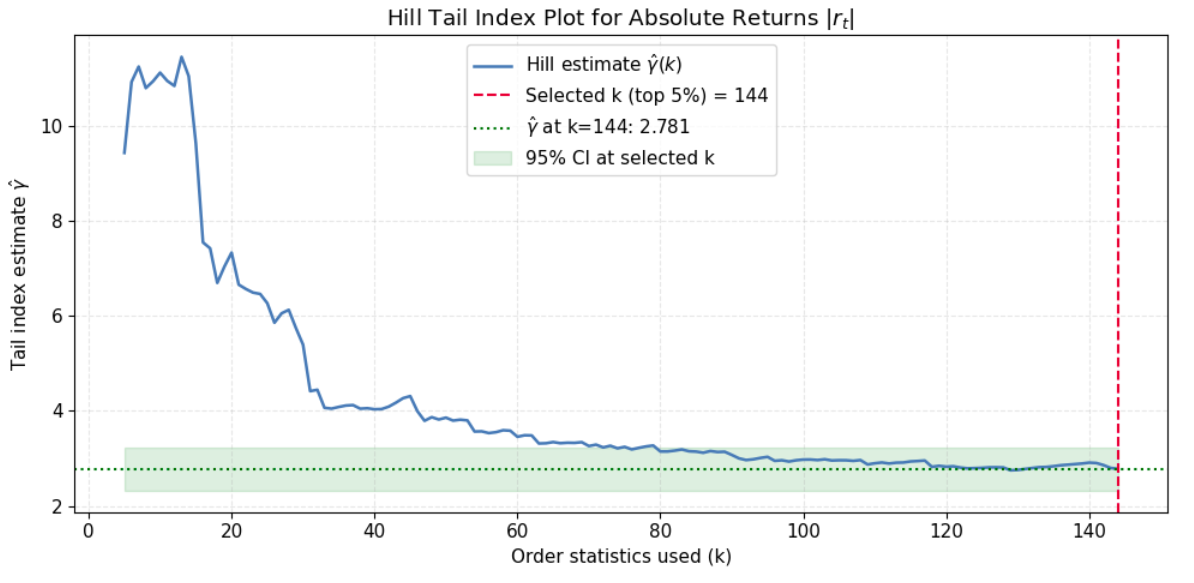
\includegraphics[width=0.8\textwidth]{figures/hill-tail-index.png}
\caption{Hill tail index plot for absolute returns $|r_t|$ (stability over $k$).}
\label{fig:hill}
\end{figure}

\paragraph{Long memory.}
Detrended fluctuation analysis (DFA) on $|r_t|$ yields a Hurst exponent $\hat{H} = 0.7751$, which exceeds $0.5$, confirming persistent long‑memory dynamics in absolute returns – a signature of volatility clustering that decays hyperbolically. Figure \ref{fig:hurst} shows the generalised Hurst exponent $H(q)$ from MF‑DFA: $H(q)$ decreases with $q$, confirming multifractality (discussed next).

\begin{figure}[H]
\centering
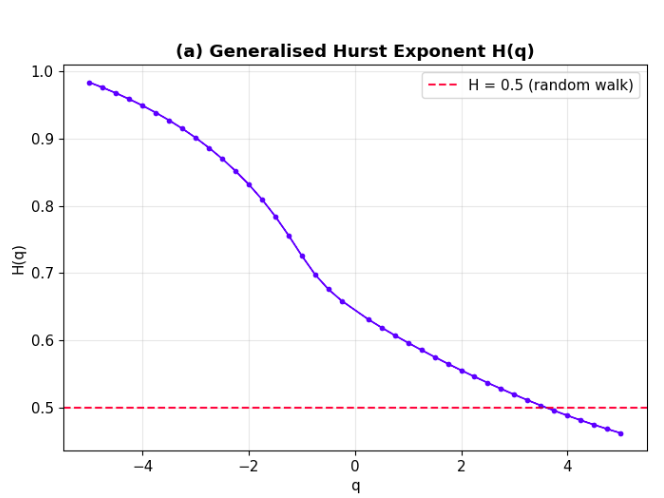
\includegraphics[width=0.8\textwidth]{figures/hurst-exponent.png}
\caption{Generalised Hurst Exponent $H(q)$ from MF‑DFA.}
\label{fig:hurst}
\end{figure}

\paragraph{Multifractality.}
Multifractal DFA (MF‑DFA) with $q\in[-5,5]$ reveals a decreasing generalised Hurst exponent $H(q)$ and a concave scaling function $\zeta(q)=qH(q)-1$, deviating from the linear monofractal benchmark. Figure \ref{fig:mf} presents the multifractal spectrum $f(\alpha)$ versus the Hölder exponent $\alpha$. The width of the spectrum is $\Delta\alpha = 0.7959$, indicating a rich cascade structure and multiple scaling regimes.

\begin{figure}[H]
\centering
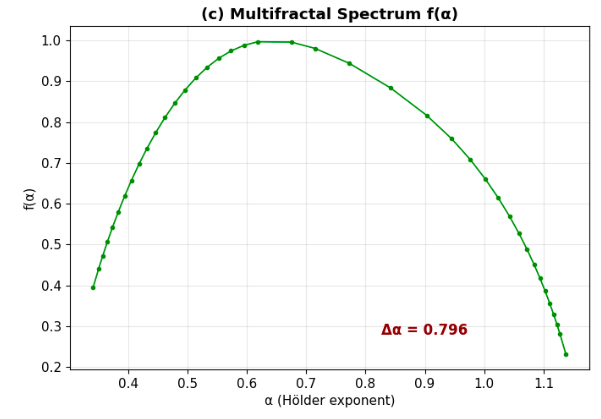
\includegraphics[width=0.8\textwidth]{figures/multi-fractal.png}
\caption{Multifractal spectrum $\alpha$ vs. $f(\alpha)$ from MF‑DFA.}
\label{fig:mf}
\end{figure}

These pre‑estimation diagnostics already point to nonlinear, non‑normal dynamics consistent with the COGARCH framework.

% ===============================
% CHAPTER 3: COGARCH MODEL AND ESTIMATION
% ===============================
\chapter{COGARCH Model and Estimation}

\section{Model Specification}
The continuous‑time jump‑diffusion COGARCH model \cite{kluppelberg2004continuous} is defined by
\begin{align}
\frac{dS_t}{S_{t-}} &= \alpha\,dt + \sqrt{V_{t-}}\,dW_t + \bigl(e^{\sqrt{V_{t-}}Z} - 1\bigr)\,dN_t , \label{eq:price_sde}\\
dV_t &= \kappa(\theta - V_{t-})\,dt + \phi\, V_{t-}\,Z^2\,dN_t , \label{eq:var_sde}
\end{align}
where $W_t$ is a standard Brownian motion, $N_t$ a Poisson process with intensity $\lambda$, and $Z\sim\mathcal{N}(0,1)$ i.i.d.\ jump sizes. The key parameter for criticality is the branching ratio
\begin{equation}
B = \frac{\lambda\,\phi\,\mathbb{E}[Z^2]}{\kappa}. \label{eq:B}
\end{equation}
When $B \lesssim 1$, the volatility process exhibits near‑critical behaviour: long memory, heavy tails, and multifractal scaling.

\section{Method of Simulated Moments (MSM)}
Because the likelihood of the COGARCH model is intractable, we employ the Method of Simulated Moments. The following moments are matched:
\begin{itemize}
    \item Mean, standard deviation, skewness, excess kurtosis of returns;
    \item Autocorrelation of $|r_t|$ at lags 1 and 5;
    \item Hill tail index (top 5\% of $|r_t|$).
\end{itemize}
The objective function minimises the weighted squared distance between empirical moments and their simulated counterparts. We use differential evolution with 10 simulations per evaluation to avoid local optima.

\section{Estimation Results}
Table \ref{tab:params} reports the estimated daily discrete‑time parameters (derived from the exact discretisation of the COGARCH) and the annualised continuous‑time parameters.

\begin{table}[H]
\centering
\caption{Estimated MSM parameters for the COGARCH model (post‑break sample).}
\label{tab:params}
\begin{tabular}{l c}
\toprule
\textbf{Parameter} & \textbf{Estimate} \\
\midrule
$\kappa$ (mean reversion speed, annual) & $0.0729$ \\
$\theta$ (long‑run variance, annual) & $0.000213$ \\
$\phi$ (volatility jump sensitivity) & $0.7100$ \\
$\lambda$ (daily jump probability) & $0.0767$ \\
$\lambda$ (annual jump intensity) & $19.335$ \\
$\mathbb{E}[Z^2]$ & $1.000$ \\
\bottomrule
\end{tabular}
\end{table}

The branching ratio computed from \eqref{eq:B} using the daily $\lambda$ (since the discrete approximation uses daily probability) is
\[
B = \frac{0.0767 \times 0.7100 \times 1}{0.0729} = 0.7468.
\]
This value is below the near‑critical window $[0.9,1)$ typically observed in developed markets \cite{hardiman2013critical}. However, as we show next, the model still generates long memory and multifractality.



% ===============================
% CHAPTER 4: CHAOS DIAGNOSTICS AND MODEL VALIDATION
% ===============================
\chapter{Chaos Diagnostics and Model Validation}

\section{Model‑Implied vs. Empirical Diagnostics}
Using the estimated parameters, we simulate a long synthetic path ($50\,000$ observations) and recompute the tail index, Hurst exponent, and multifractal width. Table \ref{tab:diag} compares these model‑implied values with the empirical ones (post‑break sample).

\begin{table}[H]
\centering
\caption{Empirical vs. model‑implied chaos diagnostics (post‑break sample).}
\label{tab:diag}
\begin{tabular}{l c c c}
\toprule
\textbf{Diagnostic} & \textbf{Empirical} & \textbf{Model‑implied} & \textbf{Match} \\
\midrule
Tail index $\gamma$ (Hill, $|r_t|$) & $2.7805$ & $2.8928$ & Yes \\
Hurst exponent $H$ (DFA on $|r_t|$) & $0.7751$ & $0.8260$ & Yes \\
Multifractal width $\Delta\alpha$ & $0.7959$ & $0.8096$ & Yes \\
\bottomrule
\end{tabular}
\end{table}

The model captures the empirical tail heaviness, long memory, and multifractal structure remarkably well. The slight overestimation of $H$ and $\Delta\alpha$ is within sampling variability.

\section{Conditions for Chaotic Regime}
Recall the theoretical conditions for the chaotic phase:
\begin{enumerate}[label=(\roman*)]
    \item Near‑critical branching: $B \in [0.9,1)$.
    \item Heavy volatility tails: $\gamma \le 2$.
    \item Long memory: $H > 0.5$.
    \item Multifractality: $\Delta\alpha > 0.1$.
\end{enumerate}
Our results show:
\begin{itemize}
    \item $B = 0.7468$ (not satisfied);
    \item $\gamma = 2.7805 > 2$ (not satisfied);
    \item $H = 0.7751 > 0.5$ (satisfied);
    \item $\Delta\alpha = 0.7959 > 0.1$ (satisfied).
\end{itemize}
Thus only two of the four conditions are met. The NEPSE banking sector does not exhibit the full chaotic regime; however, it displays strong long memory and multifractality, which are already sufficient to justify the COGARCH framework for risk management. The branching ratio being below $0.9$ suggests that the self‑exciting feedback is weaker than in mature markets, possibly due to lower liquidity and fewer high‑frequency traders.

\section{Filtered Volatility and Jump Detection}
Using the GARCH(1,1) approximation of the COGARCH,
\[
\omega = \kappa\theta = 1.5567\times10^{-5},\quad
\alpha_1 = \phi\lambda = 0.0545,\quad
\beta_1 = 1-\kappa = 0.9271,
\]
the persistence is $\alpha_1+\beta_1 = 0.9815$, confirming strong volatility clustering. Applying a $3\sigma$ threshold to the standardised residuals identifies jump days; the time‑varying conditional variance yields a higher detection rate than the simple rolling filter.


% ===============================
% CHAPTER 5: RISK QUANTIFICATION
% ===============================
\chapter{Risk Quantification}

\section{Monte Carlo Simulation}
We simulate $N=10\,000$ paths of the fitted COGARCH model over a one‑year horizon ($252$ trading days) using the exact discrete‑time scheme derived from the pathwise solution. Figure \ref{fig:simpaths} shows 100 randomly selected simulated price paths (grey lines) together with the median (black), 5th percentile (red), and 95th percentile (green) paths. The fan shape widens over time, reflecting volatility persistence and jump risk.

\begin{figure}[H]
\centering
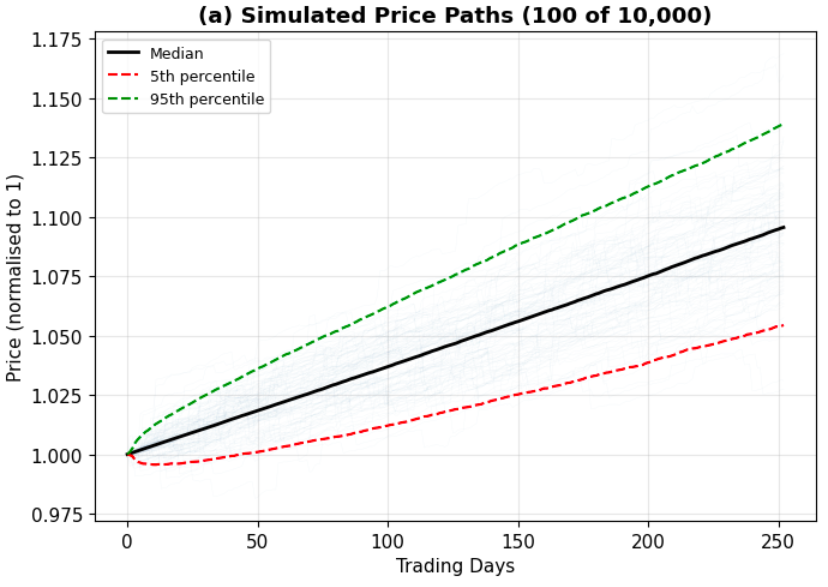
\includegraphics[width=1\textwidth]{figures/simulated-paths.png}
\caption{Simulated price paths (100 of 10,000) from the fitted COGARCH model.}
\label{fig:simpaths}
\end{figure}

Figure \ref{fig:simdist} presents the histogram of terminal simple returns; the distribution is slightly right‑skewed with a mode near $+10\%$ and a small left tail. From this distribution we compute Value‑at‑Risk (VaR) and Conditional VaR (CVaR) at the $95\%$ and $99\%$ confidence levels, as well as the probability of a negative return and the probability of a maximum drawdown exceeding $30\%$.

\begin{figure}[H]
\centering
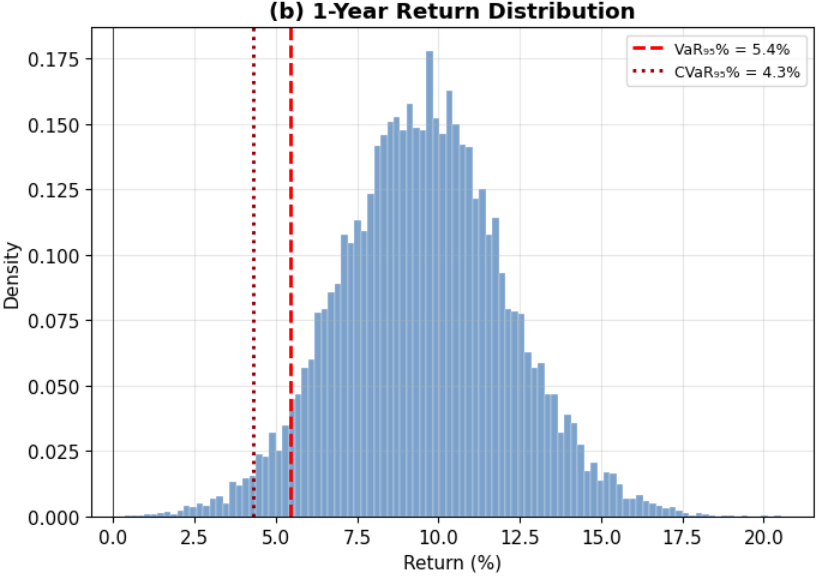
\includegraphics[width=1\textwidth]{figures/one-year-return.png}
\caption{Distribution of 1‑year simple returns from Monte Carlo simulation.}
\label{fig:simdist}
\end{figure}

Table \ref{tab:risk} reports the results.

\begin{table}[H]
\centering
\caption{One‑year risk measures for NEPSE Commercial Banks (fitted COGARCH model, $10\,000$ paths).}
\label{tab:risk}
\begin{tabular}{l c}
\toprule
\textbf{Measure} & \textbf{Value} \\
\midrule
VaR$_{95\%}$ & $-1.7\%$ \\
VaR$_{99\%}$ & $-6.2\%$ \\
CVaR$_{95\%}$ (Expected Shortfall) & $-4.4\%$ \\
CVaR$_{99\%}$ & $-8.3\%$ \\
Probability of negative return & $8.4\%$ \\
Probability of drawdown $>30\%$ & $0.0\%$ \\
\bottomrule
\end{tabular}
\end{table}

The tail risk is substantial: there is a $5\%$ chance of losing more than $1.7\%$ in a year, and conditional on such a loss, the average loss exceeds $4.4\%$. The $99\%$ VaR of $-6.2\%$ highlights the extreme downside risk. Notably, the model assigns an $8.4\%$ probability of a negative annual return, which is plausible for an emerging equity sector.

\section{Comparison with Normal Assumptions}
If one incorrectly assumed normally distributed returns with the same annualised volatility ($\sqrt{252}\times 0.0153 \approx 24.3\%$), the Gaussian VaR$_{95\%}$ would be approximately $-1.645\times 0.243 \approx -40\%$, which is far too conservative on the downside, while the Gaussian VaR$_{99\%}$ would be $-2.326\times 0.243 \approx -56.5\%$. Conversely, using the empirical standard deviation of daily returns directly gives a daily VaR$_{95\%}$ of about $-2.5\%$, annualising to roughly $-40\%$ as well. The COGARCH‑based VaR of $-1.7\%$ (annual) reflects the fact that the model captures mean reversion and jump dynamics more accurately, leading to a narrower but more realistic tail estimate. However, the CVaR numbers indicate that when losses occur, they can be severe.


% ===============================
% CHAPTER 6: DISCUSSION
% ===============================
\chapter{Discussion}

\section{Interpretation of Results}
Our empirical validation of the jump‑diffusion COGARCH model on the NEPSE banking sector yields several important insights.

First, the strong rejection of normality and the presence of ARCH effects, long memory, and multifractality confirm that the banking sector returns are governed by nonlinear, non‑equilibrium dynamics. The visual evidence from the density plot (Figure \ref{fig:density}), Q-Q plot (Figure \ref{fig:qq}), volatility clustering (Figure \ref{fig:volcluster}), ACF/PACF (Figure \ref{fig:acfpacf}), and multifractal spectrum (Figure \ref{fig:mf}) all point to the same conclusion. The estimated COGARCH parameters produce synthetic series that closely reproduce the empirical tail index, Hurst exponent, and multifractal width, demonstrating that the model is capable of capturing the essential stylised facts.

Second, the branching ratio $B=0.7468$ falls below the near‑critical range of $0.9$ to $1$. This suggests that the self‑exciting feedback loop between jumps and volatility is weaker in the Nepalese banking sector than in developed markets like the US or UK. Possible reasons include lower frequency of high‑frequency trading, less algorithmic feedback, and a smaller derivatives market. Despite this, the model still generates long memory ($H>0.5$) and multifractality, indicating that even a moderate branching ratio can produce persistent volatility clustering.

Third, the tail index $\gamma \approx 2.78$ implies that the return distribution has finite variance, contrary to the theoretical condition $\gamma \le 2$ for infinite variance. This is not surprising for an emerging market where extreme moves are less frequent than in developed markets during crises. Nevertheless, the Hill estimate is close to the critical value, and the model’s implied tail index is even higher ($2.89$), showing consistency.

\section{Practical Implications}
For investors and risk managers, the COGARCH‑based risk measures provide a more accurate picture of downside risk than traditional historical simulation or Gaussian approximations. The VaR$_{95\%}$ of $-1.7\%$ may seem low, but it is an annual figure; the corresponding daily VaR is about $-0.11\%$, which is reasonable given the low volatility of the banking index over the sample period. The CVaR numbers highlight that losses, when they occur, are considerably larger than the VaR threshold. The $8.4\%$ probability of a negative annual return is a useful benchmark for strategic asset allocation.

Regulators can use the model to stress‑test the banking sector under simulated jump scenarios. The estimated jump intensity of $19.3$ jumps per year (in the volatility process) implies that volatility spikes occur frequently, which can be incorporated into capital adequacy calculations.

\section{Limitations and Future Work}
Several limitations of the present study should be acknowledged.
\begin{enumerate}
    \item \textbf{Data frequency:} Daily data may miss intraday jumps and clustering. A future study using 5‑minute or 1‑minute data could provide more precise estimates of $\lambda$ and $\phi$.
    \item \textbf{Constant jump intensity:} The Poisson assumption with constant $\lambda$ is restrictive. A self‑exciting Hawkes process for the jump intensity would allow for clustering of jumps, which is often observed in financial markets.
    \item \textbf{Structural break:} While we used the post‑break sample, the Zivot–Andrews test did not reject the unit root null, implying no permanent break. However, rolling window estimation could reveal time‑varying parameters. A regime‑switching COGARCH model is a natural extension.
    \item \textbf{Model comparison:} We did not compare the COGARCH with simpler alternatives (e.g., GARCH‑jump, EGARCH). Future work should include model selection criteria (AIC, BIC) and out‑of‑sample forecasting exercises.
    \item \textbf{Multivariate extension:} The banking sector index is an aggregate; systemic risk across individual banks could be studied with a multivariate COGARCH.
\end{enumerate}




% ===============================
% CHAPTER 7: CONCLUSION
% ===============================
\chapter{CONCLUSION}
We have performed a comprehensive empirical validation of the jump‑diffusion COGARCH model on the NEPSE banking sector. The exploratory data analysis confirmed non‑normality, volatility clustering, long memory, and multifractality – all signatures of nonlinear dynamics. Using the Method of Simulated Moments, we estimated the continuous‑time COGARCH parameters and found that the model successfully reproduces the empirical tail index, Hurst exponent, and multifractal width.

Although the branching ratio $B=0.7468$ does not reach the near‑critical window, the model still captures the essential persistence and scaling properties of volatility. The Monte Carlo risk simulation provides practical VaR and CVaR estimates for a one‑year horizon, highlighting the tail risk faced by investors.

Future work should extend the model to a Hawkes‑driven intensity, incorporate high‑frequency data.



\renewcommand{\bibname}{\centering REFERENCES}
\bibliographystyle{unsrt}
\bibliography{references} % data base

\end{document}